\subsection*{}
Los datos se consideran accesibles por el usuario cuando este no necesita realizar un esfuerzo desmesurado para
poder obtenerlos, entenderlos y usarlos, es decir, aplicarlos a su situacion particular. Para lograr estos objetivos,
es necesario que el usuario pueda acceder a ellos de una manera que le resulte familiar y en un lenguage y nomenclatura
que pueda entender.\\ 

En este apartado veremos si es posible el acceso a los datos por un usuario medio y como optimizar la accesibilidad.
\subsection{Disponibilidad vs Accesibilidad}
    
Como mencionamos en la introduccion de este capitulo, los datos pueden estar disponibles en la fuente original, pero no por
ello significa que estos sean accesibles.
Los retos a los que nos encontramos con los datos crudos, directos de la fuente de origen, son los siguientes:
    
    \begin{itemize}
        \item \textbf{Localizacion}. Los datos se encuentran disponibles en portales de datos abiertos organizados 
        y estructurados, normalmente se necesita una tarea de busqueda y seleccion
        a veces complicada. Aunque las empresas ponen cada vez mas de su parte en ofrecer una interfaz 
        agradable y funcional a los usuarios, esta tarea requiere de un trabajo de investigacion por parte del usuario,
        ya que posiblemente, debera buscar en distintos portales.
        \item \textbf{Accesibilidad}. Los datos suelen estan disponibles a traves de una interfaz de programacion 
        de aplicaciones (API) no facilmente interpretable por el usuario medio. Normalmente cuenta con 
        un documento que describe cada uno de los campos y valores que se presentan en el documento y como utilizar la API.
        \item \textbf{Interpretabilidad}. Usualmente los datos estan representados en un formato para ser procesado por 
        algun software, por lo que su lectura resulta complicada por el usuario medio, en el mejor de los casos, 
        estaran representados en una tabla y aun asi, sera muy dificil de extraer informacion.
        \item \textbf{Almacenamiento}. Los datos publicados son los mas recientes, por lo que no hay manera de obtener 
        un historico de los datos si no son almacenados periodicamente. Una vez extraidos los datos, el usuario debera 
        contar con una infraestructura que le permita almacenar los datos.
        \item \textbf{Automatizacion}. Este proceso tiende a ser arduo, por lo que sera necesario automatizarlo, de otra 
        forma el esfuerzo requerido por el usuario para extraer la informacion no le compensara.
         
    \end{itemize}
    
Por lo tanto, no podemos decir que estos datos sean accesibles de una forma util para el usuario medio.\\

\subsection{Interpretacion de los datos}

Recordemos que el objetivo principal del acceso a los datos, es obtener conocimiento. Hay que tener en 
cuenta que los datos por si solos, no tienen ningun valor, ya que carecen de sentido, una vez integrados en un contexto,
nos aportara informacion, y procesando y analizando esta informacion, se obtendra el conocimiento.\\
    
\begin{figure}[h]
    \centering 
    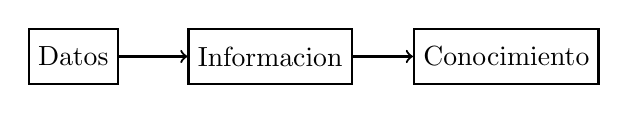
\begin{tikzpicture}[thick]
        \node[draw,rectangle,minimum size=20] (a) {Datos};
         \node[draw,rectangle,minimum size=20,right of= a, node distance=2.5cm] (b) {Informacion};
         \node[draw,rectangle,minimum size=20,right of=b, node distance=3cm] (c) {Conocimiento};
         \draw[->] (a) to (b);
        \draw[->] (b) to (c);
     
      \end{tikzpicture}
      \caption{Diagrama. De datos a conocimiento}
    \end{figure}
 
Para poder obtener este conocimiento de los datos, es necesario que el usuario interprete correctamente los datos, por lo
que el usuario debe contar con conocimientos en la materia o realizar una tarea de investigacion, que le permita 
entender los datos extraidos. \\

Asi pues, para que el usuario pueda obtener la informacion de una manera directa, requiere de conocimientos tanto 
de programacion como especificos de la materia y los recursos para crear una infraestructura que le permita implementar 
una representacion de los datos que le sea util.\\

Podemos concluir que el acceso a los datos por parte del usuario medio, no es directa.\\

Para poder construir un sistema que haga los datos accesibles, es imprescindible disenar un modelo  para concretar la 
informacion que se desea obtener. El diseno de un sistema permitira que a partir de unos valores dados, proporcione unos resultados.
Para ello sera necesario tener un conocimiento solido del conjunto de datos que se necesita, los valores,
sus unidades y como se relacionan entre si\\
    
\subsection{Formato}

Los datos proporcionados por las plataformas tienen un gran volumen, ya que como comentabamos anteriormente, se recolectan
el mayor numero de datos posibles.Este documento contara con multiples muestras para las que
se especifica un conjunto campos. Estos conjuntos de campos son similares entre ellos, pero no tienen por que ser identicos. 
De estos datos, se debera realizar una seleccion de las muestras relevantes, y de estas, los campos necesarios
para su diseno y cuales no.
\newpage

A continuacion podemos ver varios ejemplos tomados del portal de datos abiertos europeo
\footnote{\url{https://tinyurl.com/y3d76525}} 
y norte americano\footnote{\url{https://data.cityofnewyork.us/api/views/kku6-nxdu/rows.json?accessType=DOWNLOAD}}.

\begin{figure}[h]
    \centering
    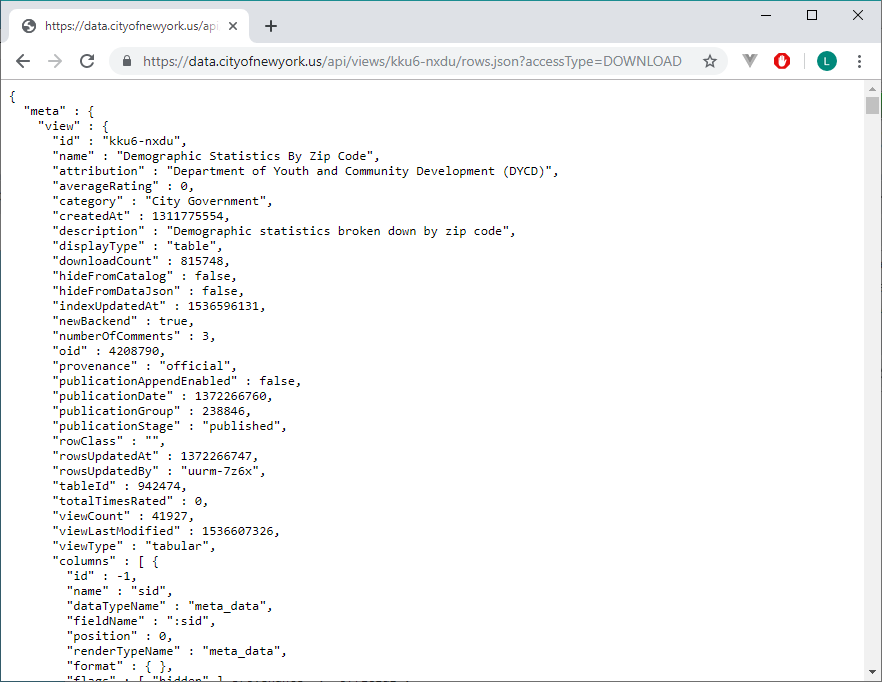
\includegraphics[width=8cm]{ExampleOpenData1}
    \caption{EEUU Open Portal.Demographic Statistics By Zip Code}
    \end{figure}

    \begin{figure}[h]
    \centering
    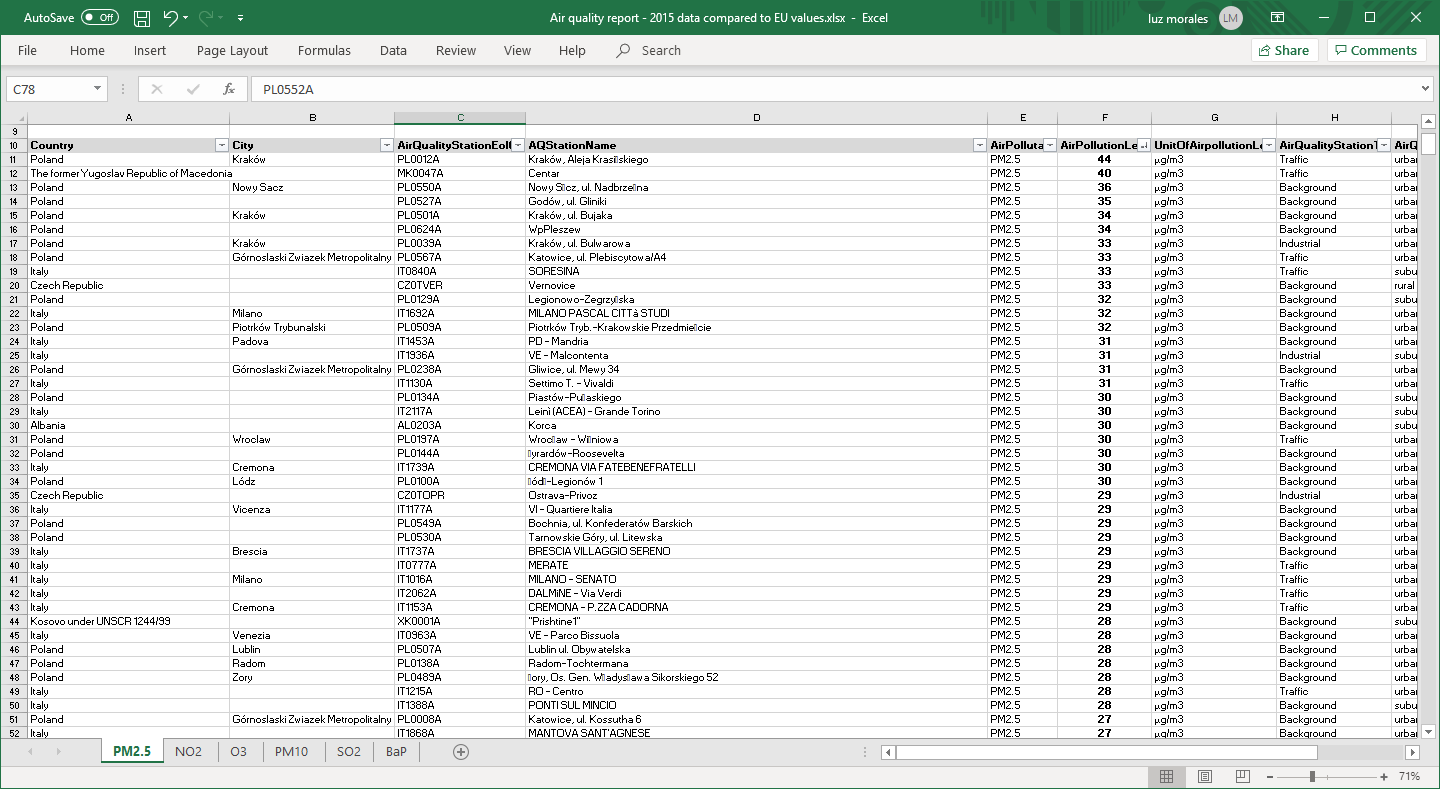
\includegraphics[width=11.5cm]{ExampleOpenData2}
    \caption{European Open Portal. Air pollutant concentrations 2015} 
   
 
\end{figure}

\newpage
    
A traves de una serie de procesos como son  la extraccion, transformacion y 
limpieza de los datos, se obtendran los datos que se necesitan acorde a nuestro diseno. Estos procesos pueden llegar
a ser muy tediosos si no se automatizan.
Veremos estos procesos en los siguientes apartados\\
    

\subsection{Optimizacion de la accesibilidad}

Para ofrecer los datos a los usuarios de una manera directa, es recomendable utilizr una plataforma a la que el usuario
este familiarizado. Por ejemplo, es mas factible que el usuario se sienta mas atraido a acceder a los datos si no requiere
ninguna instalacion en sus dispositivos.

\begin{comment}
    

    ----Respecto a polucion del aire 
    Acudir a fuentes privadas
    Instalacion de dispositivos
  Done-  Ejemplos de bases de datos de distintas ciudades capitales


    --no plataformas de pago
Done -no instalacion de software
-no complicaciones por parte del usuario.

--Datos automatizados -- formato maquina
--almacenamiento
--conocimientos informaticos
--analiticos
--estudio de la materia, ver que es importante o no, contrastarlo
--equipo multidisciplinario
--informaticos no son expertos en medicina, por ejemplo.
\begin{itemize}

    \item datos disponible
    \item no substraible por el usuario medio
    \item imposible de tratar sin una estructura
    \item no es posible de tener un historico
    \item sin informacion complementaria que muestre informacion util
    \item Desperdicio
    \item \end{itemize}

---Si fuera necesario, se le puede proporcionar las herramientas para que pueda entenderlo, en los 
casos mas complicados donde se necesitan conocimientos previos sobre la materia.

---Incluir concepto de muestras
\end{comment}  
    